\chapter{Calculating Temperature Changes using the fMRI BOLD Response}

\section{Background}
  % What does the BOLD response tell us?
  % What gives rise to the fMRI BOLD response?
  \subsection{Generation of the {B}lood {O}xygen {L}evel {D}ependent ({BOLD}) Response}
    \begin{figure}
      \begin{center}
        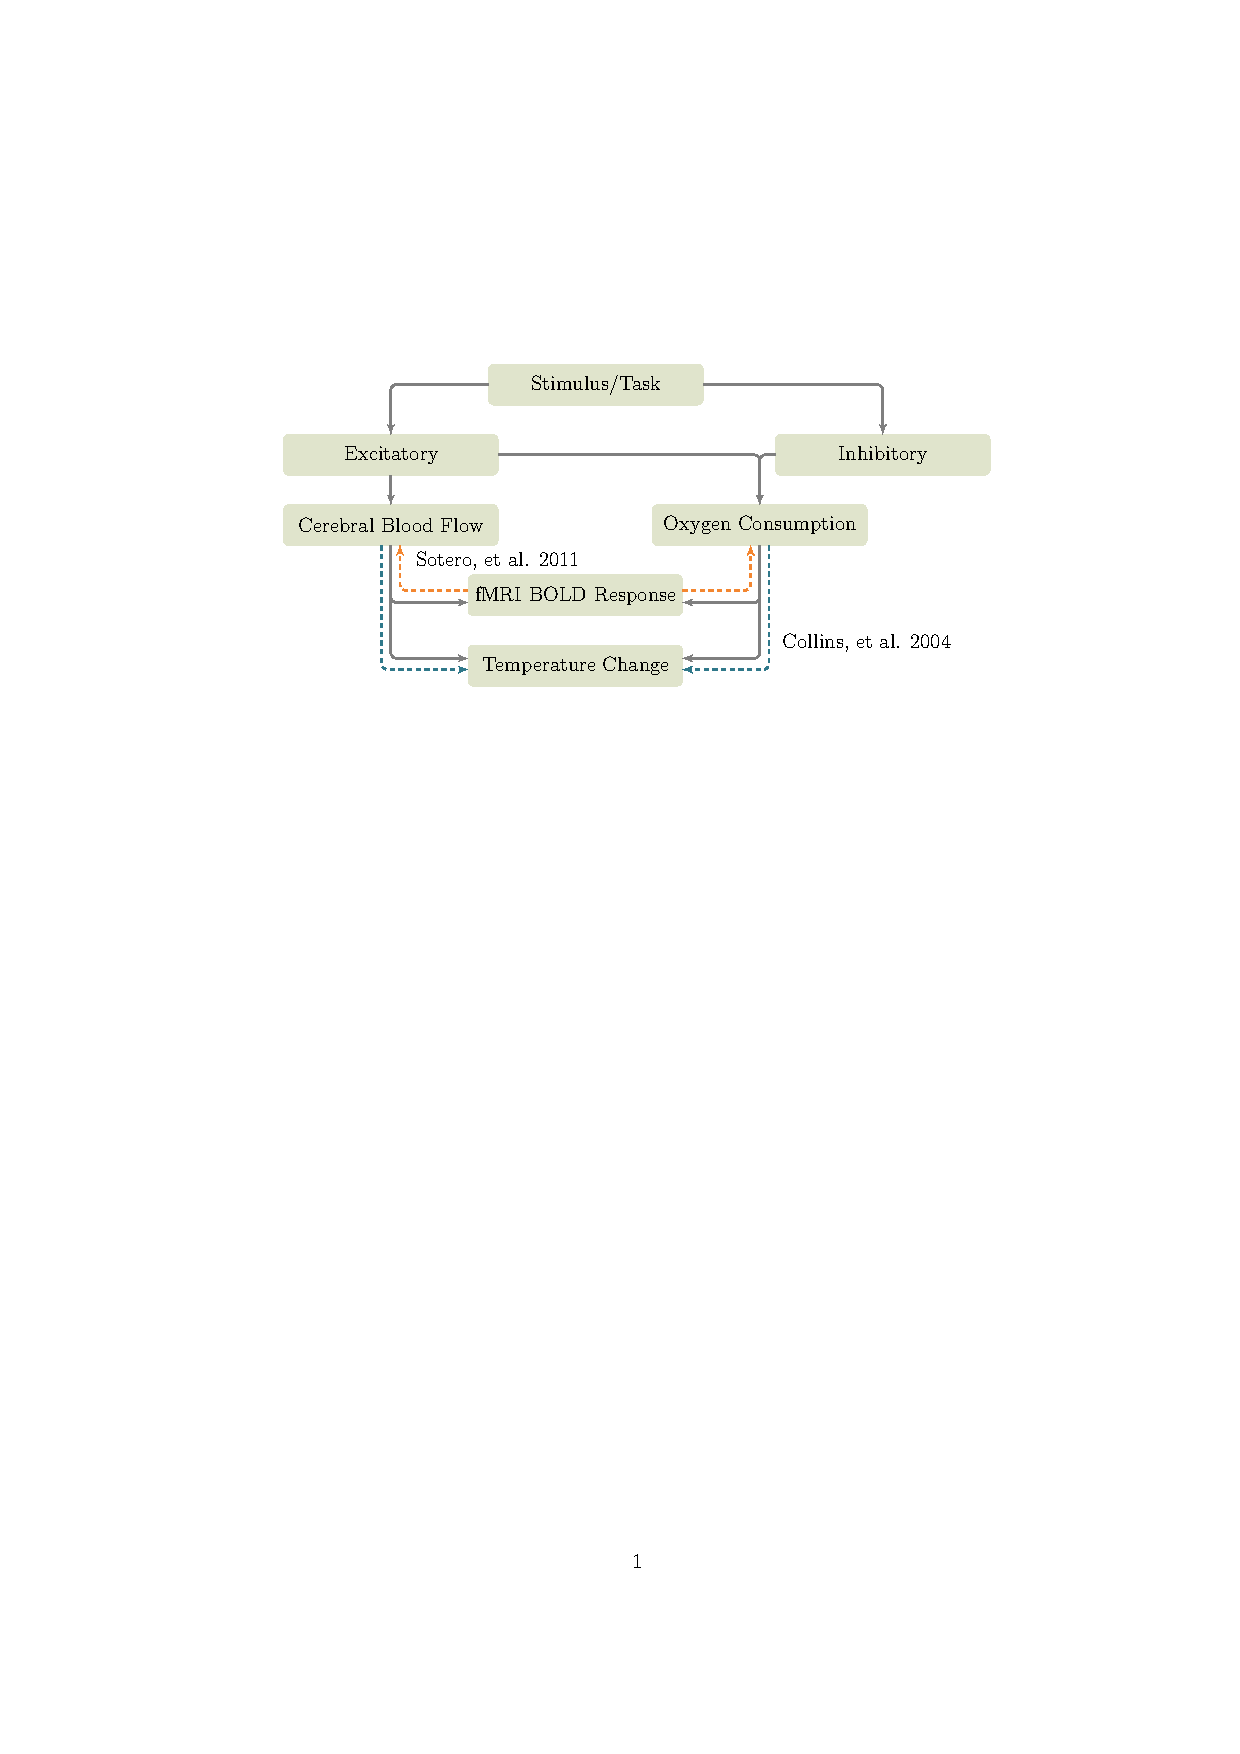
\includegraphics{flowchart}
        \caption[Generation of the fMRI BOLD Response]{\label{fig:flowchart} Generation of the fMRI BOLD response from changes in neuronal activity.  Black arrows indicate a causal relationship while red arrows indicate existing models for the relationship.  Modified from~\citet{sotero2007}}
      \end{center}
    \end{figure}
    
  \subsection{Previously Proposed Temperature Models}
  Current efforts to model temperature changes be can categorized into two classes.  The first class approaches the problem by considering a single voxel deep within the brain (single-voxel approach) while the second approach considers the brain and head as an entire system (multi-voxel approach).  Each of these methods has their own pros and cons which will be discussed below.
    \subsubsection{\label{sss:singlevoxel}Single-Voxel Approach}
    A single-voxel model of temperature was first proposed by SOMEONE, but has been refined over the past HOWLONG years CITEABUNCH to include more terms.  Although different approaches consider different contributions to the temperature change, they all narrow the problem down to a single voxel which is usually 2mm x 2mm x 2mm.  By simplifying the model, the heat equation can be simplified and the calculation is much easier to undertake.  However, since the brain is not homogenous, the values used for parameters such as heat production and thermal conductivity are taken from an average of the tissues.  As a result, this reduces the possible accuracy of such a model when applied to a subject.
    The most recently published iteration of a single-voxel model was published by~\citet{sotero2011}.  The basis of this model is a modification of the Penne's Bioheat Equation~\citep{pennes}.
    %%%%%%%  Bio-heat Equation %%%%%%%%%%%%
    \begin{equation}
      C_t \frac{dT(t)}{dt} = (\Delta H^{\circ}-\Delta H_{b}) CMRO_{2}\mid_{0} m(t) - \rho_{b} C_{b} CBF\mid_{0} f(t) (T(t) - T_{a}) - \frac{C_{t}}{\tau} (T(t)-T_{0})
    \end{equation}
    %%%%%%%%%%%%%%%%%%%%%%%%%%%%%%%%%%%%%%%%
    where BLA BLA BLA.  While complicated in symbol, conceptually the equation can be easily understood.
    %%%%%%%  Explanation %%%%%%%%%%%%%%%%%%%
    \begin{equation}    change~in~temperature~=~heat~generated~by~metabolism~-~heat~lost~to~convection~-~heat~lost~to~conduction
    \end{equation}
    %%%%%%%%%%%%%%%%%%%%%%%%%%%%%%%%%%%%%%%%
    \subsubsection{\label{sss:multivoxel}Multi-Voxel Approach}
  


\section{Modeling the BOLD Response}
% Start with Buxton and Friston and build up to how I am calculating the metabolism and blood flow.

\section{Modeling Temperature}
  % go through the other approaches
  \subsection{The Approach}
    \subsubsection{How the temperature is calculated}
    \subsubsection{Calculating the equilibrium temperature}
    \subsubsection{Calculating Metabolism and Blood Flow Changes}
    \subsubsection{Calculating the change in temperature in the active brain}
  \subsection{Results}
    \subsubsection{Using Theoretical BOLD Data}
    \subsubsection{Using Experimental BOLD Data}
  % talk about my approach